\documentclass{article}

\usepackage[utf8]{inputenc}
\usepackage{longtable}
\usepackage{authblk}
\usepackage{adjustbox}
\usepackage{natbib}



\title{LOS ÍNDICES DE COLOMBIA}
% autores
\author[1]{\normalsize Sara Barón}
\affil[1]{\small  Escuela de Ingeniería,Universidad de los Andes\\
\texttt{{sj.baron10}@uniandes.edu.co}}


\date{29 de Junio de 2018}

\usepackage{Sweave}
\begin{document}
\Sconcordance{concordance:ProyectoFinal.tex:ProyectoFinal.Rnw:%
1 19 1 1 0 13 1 1 6 1 1 1 5 12 1 1 5 14 0 1 2 3 1 1 10 1 3 7 1 1 11 1 3 %
7 1 1 6 12 0 1 3 6 1 1 7 1 3 9 1 1 5 1 4 31 0 1 22 1 1 1 18 6 1 1 14 1 %
2 8 1}

\maketitle


\begin{abstract}
Este es mi primer trabajo en exploración y modelamiento de indices usando LATEX. Este trabajo lo he hecho bajo la filosofía de trabajo replicable. Este es mi primer trabajo en exploración y modelamiento de indices usando LATEX. Este trabajo lo he hecho bajo la filosofía de trabajo replicable. Este es mi primer trabajo en exploración y modelamiento de indices usando LATEX. Este trabajo lo he hecho bajo la filosofía de trabajo replicable. Este es mi primer trabajo en exploración y modelamiento de indices usando LATEX. Este trabajo lo he hecho bajo la filosofía de trabajo replicable.
\end{abstract}

\section*{Introducción}

Aquí les presento mi investigación sobre diversos indices sociales en el mundo. Los indices los conseguí de wikipedia, espero que les gusten mucho. Aquí les presento mi investigación sobre diversos indices sociales en el mundo. Los indices los conseguí de wikipedia, espero que les gusten mucho.Aquí les presento mi investigación sobre diversos indices sociales en el mundo. Los indices los conseguí de wikipedia, espero que les gusten mucho.Aqui les presento mi investigación sobre diversos indices sociales en el mundo. Los indices los conseguí de wikipedia, espero que les gusten mucho.
Aquí les presento mi investigacion sobre diversos indices sociales en el mundo. Los indices los conseguí de wikipedia, espero que les gusten mucho.Aqui les presento mi investigacion sobre diversos indices sociales en el mundo. Los indices los conseguí de wikipedia, espero que les gusten mucho.Aqui les presento mi investigacion sobre diversos indices sociales en el mundo. Los indices los conseguí de wikipedia, espero que les gusten mucho.





%Exploracion Univariada

Comencemos viendo que hay en la sección \ref{univariada} en la página \pageref{univariada}.

\clearpage

\section{Exploración Univariada}\label{univariada}

En esta sección exploro cada índice. En esta sección exploro cada índice. En esta sección exploro cada índice. En esta sección exploro cada índice. En esta sección exploro cada índic. En esta sección exploro cada ??ndice. En esta sección exploro cada índice. En esta sección exploro cada índice. En esta sección exploro cada índice. En esta sección exploro cada índice. En esta sección exploro cada índice. En esta sección exploro cada índice. En esta sección exploro cada índice. En esta sección exploro cada índice. En esta sección exploro cada índice. En esta sección exploro cada índice. En esta sección exploro cada índice. En esta sección exploro cada índice. En esta sección exploro cada índice. En esta sección exploro cada índice. En esta sección exploro cada índice.

%Estadísticos
% Table created by stargazer v.5.2.2 by Marek Hlavac, Harvard University. E-mail: hlavac at fas.harvard.edu
% Date and time: vie., jun. 29, 2018 - 8:11:26 p. m.
\begin{table}[!htbp] \centering 
  \caption{Medidas estadísticas} 
  \label{stats} 
\begin{tabular}{@{\extracolsep{5pt}}lcc} 
\\[-1.8ex]\hline 
\hline \\[-1.8ex] 
Statistic & \multicolumn{1}{c}{N} & \multicolumn{1}{c}{Median} \\ 
\hline \\[-1.8ex] 
IDH & 32 & 0.804 \\ 
Población.Cabecera & 32 & 717,197 \\ 
Población.Resto & 32 & 268,111.5 \\ 
\hline \\[-1.8ex] 
\end{tabular} 
\end{table} 
\begin{figure}[h]
\centering
\begin{adjustbox}{width=7cm,height=7cm,clip,trim=1.5cm 0.5cm 0cm 1.5cm}
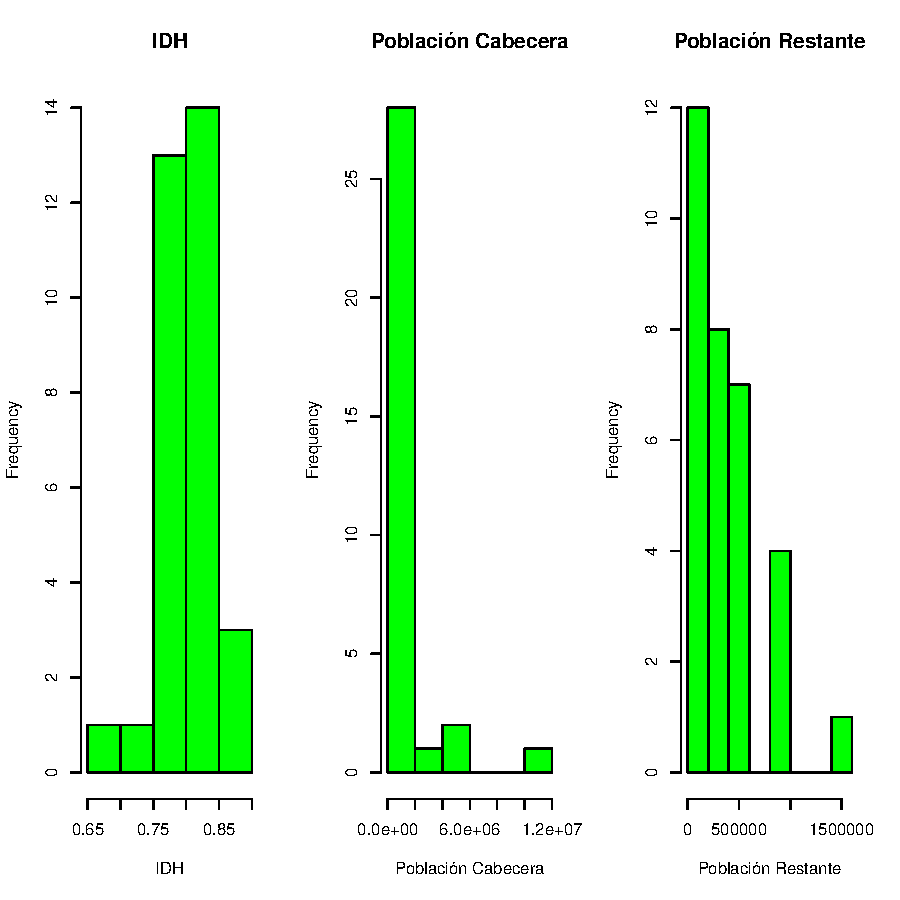
\includegraphics{ProyectoFinal-hist}
\end{adjustbox}
\caption{Histogramas}
\label{hist}
\end{figure}

Como se muestra en la figura \ref{hist} los datos no se encuentran normalizados, por ende se muestra la figura \ref{histnorm} con el fin de mejorar los datos datos se acercaron a la normalidad.Como se muestra en la figura \ref{hist} los datos no se encuentran normalizados, por ende se muestra la figura \ref{histnorm} con el fin de mejorar los datos datos se acercaron a la normalidad.

\begin{figure}[h]
\centering
\begin{adjustbox}{width=7cm,height=7cm,clip,trim=1.5cm 0.5cm 0cm 1.5cm}
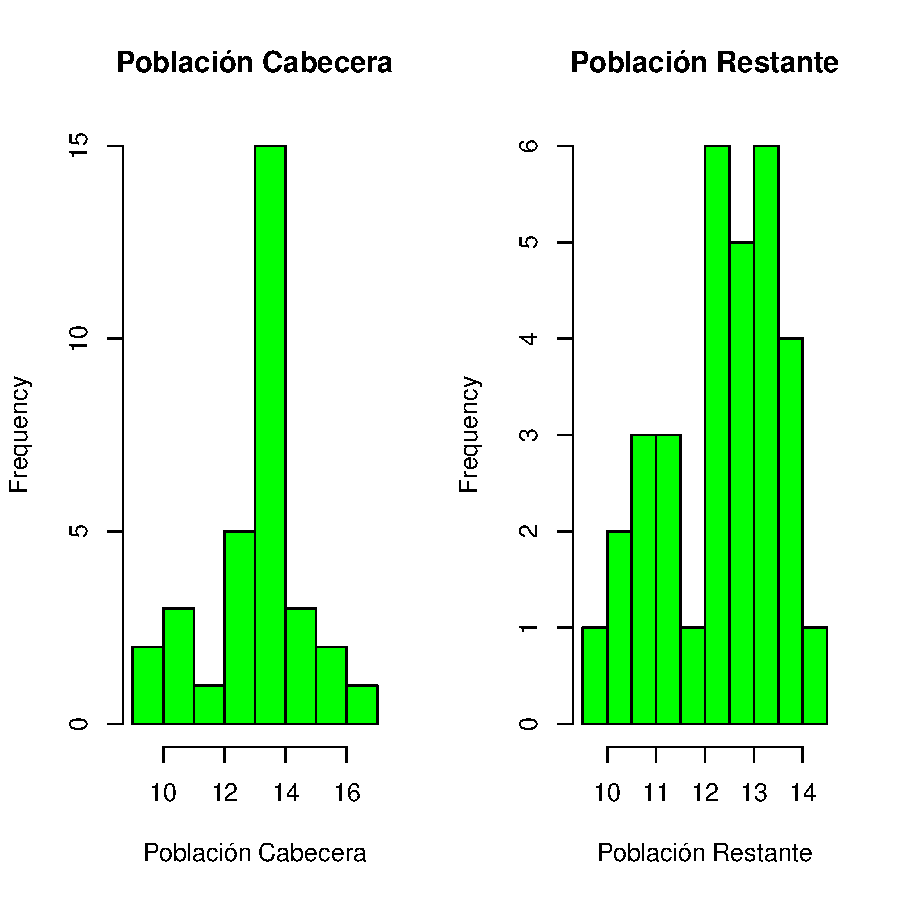
\includegraphics{ProyectoFinal-histnorm}
\end{adjustbox}
\caption{Histogramas Normalizados}
\label{histnorm}
\end{figure}

Continuamos viendo que hay en la sección \ref{bivariada} en la página \pageref{bivariada}.

\section{Exploración Bivariada}\label{bivariada}

Con el fin de obervar el impacto de la población en el IDH, obervamos el IDH con cada uno y su correlación, como se muestra en la tabla \ref{Corr}. Con el fin de obervar el impacto de la población en el IDH, obervamos el IDH con cada uno y su correlación, como se muestra en la tabla \ref{Corr}. Con el fin de obervar el impacto de la población en el IDH, obervamos el IDH con cada uno y su correlación, como se muestra en la tabla \ref{Corr}

% Table created by stargazer v.5.2.2 by Marek Hlavac, Harvard University. E-mail: hlavac at fas.harvard.edu
% Date and time: vie., jun. 29, 2018 - 8:11:26 p. m.
\begin{table}[!htbp] \centering 
  \caption{Correlación entre variables independientes} 
  \label{Corr} 
\begin{tabular}{@{\extracolsep{5pt}} ccc} 
\\[-1.8ex]\hline 
\hline \\[-1.8ex] 
 & cabeLog & restoLog \\ 
\hline \\[-1.8ex] 
cabeLog & $1$ & $0.840$ \\ 
restoLog & $0.840$ & $1$ \\ 
\hline \\[-1.8ex] 
\end{tabular} 
\end{table} 
Adicionalmente, se muestra la Correlación entre variables independientes, en la figura \ref{CorrInd}. Adicionalmente, se muestra la Correlación entre variables independientes, en la figura \ref{CorrInd}. Adicionalmente, se muestra la Correlación entre variables independientes, en la figura \ref{CorrInd}. Adicionalmente, se muestra la Correlación entre variables independientes, en la figura \ref{CorrInd}.Adicionalmente, se muestra la Correlación entre variables independientes, en la figura \ref{CorrInd}. Adicionalmente, se muestra la Correlación entre variables independientes, en la figura \ref{CorrInd}.

\begin{figure}[h]
\centering
\begin{adjustbox}{}

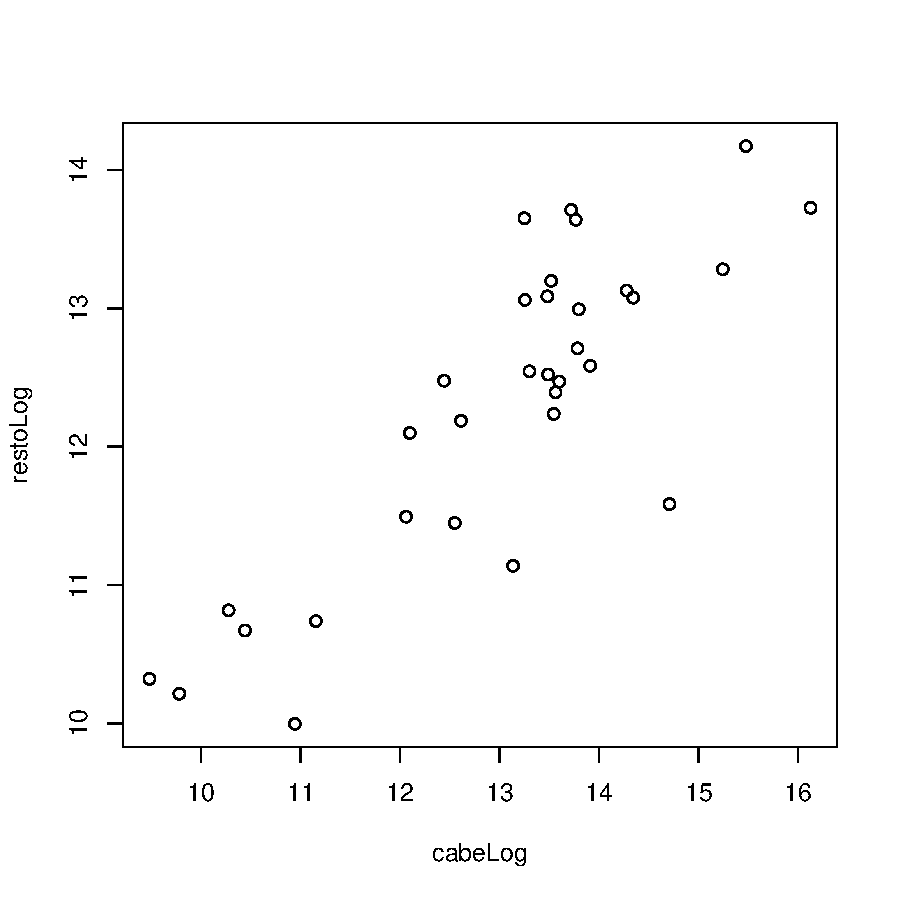
\includegraphics{ProyectoFinal-CorrInd}
\end{adjustbox}
\caption{Correlación}
\label{CorrInd}
\end{figure}

\section{Modelos de Regresión}\label{ModReg}

A continuación (\ref{regresiones}), se observan los modelos de regresión, en el primero no se tiene en cuenta la población restante y el segundo modelo ya tiene ambas variables.A continuación (\ref{regresiones}), se observan los modelos de regresión, en el primero no se tiene en cuenta la población restante y el segundo modelo ya tiene ambas variables.A continuación (\ref{regresiones}), se observan los modelos de regresión, en el primero no se tiene en cuenta la población restante y el segundo modelo ya tiene ambas variables.A continuación (\ref{regresiones}), se observan los modelos de regresión, en el primero no se tiene en cuenta la población restante y el segundo modelo ya tiene ambas variables.A continuación (\ref{regresiones}), se observan los modelos de regresión, en el primero no se tiene en cuenta la población restante y el segundo modelo ya tiene ambas variables.A continuación (\ref{regresiones}), se observan los modelos de regresión, en el primero no se tiene en cuenta la población restante y el segundo modelo ya tiene ambas variables.


% Table created by stargazer v.5.2.2 by Marek Hlavac, Harvard University. E-mail: hlavac at fas.harvard.edu
% Date and time: vie., jun. 29, 2018 - 8:11:26 p. m.
\begin{table}[!htbp] \centering 
  \caption{Modelos de Regresión} 
  \label{regresiones} 
\begin{tabular}{@{\extracolsep{5pt}}lcc} 
\\[-1.8ex]\hline 
\hline \\[-1.8ex] 
 & \multicolumn{2}{c}{\textit{Dependent variable:}} \\ 
\cline{2-3} 
\\[-1.8ex] & \multicolumn{2}{c}{IDH} \\ 
\\[-1.8ex] & (1) & (2)\\ 
\hline \\[-1.8ex] 
 cabeLog & 0.013$^{***}$ & 0.031$^{***}$ \\ 
  & (0.004) & (0.007) \\ 
  & & \\ 
 restoLog &  & $-$0.030$^{***}$ \\ 
  &  & (0.010) \\ 
  & & \\ 
 Constant & 0.634$^{***}$ & 0.766$^{***}$ \\ 
  & (0.055) & (0.065) \\ 
  & & \\ 
\hline \\[-1.8ex] 
Observations & 32 & 32 \\ 
R$^{2}$ & 0.238 & 0.425 \\ 
Adjusted R$^{2}$ & 0.212 & 0.385 \\ 
Residual Std. Error & 0.037 (df = 30) & 0.033 (df = 29) \\ 
F Statistic & 9.347$^{***}$ (df = 1; 30) & 10.706$^{***}$ (df = 2; 29) \\ 
\hline 
\hline \\[-1.8ex] 
\textit{Note:}  & \multicolumn{2}{r}{$^{*}$p$<$0.1; $^{**}$p$<$0.05; $^{***}$p$<$0.01} \\ 
\end{tabular} 
\end{table} 
\section{Exploración Espacial}\label{ExpEspa}

A continuaicón, se usara la tecnica de k-means propuesta por MacQueen \cite{macqueen_methods_nodate} para conglomerar toda la información y mostrar la información en el mapa de Colombia como se observa en \ref{clustmap}. A continuaicón, se usara la tecnica de k-means propuesta por MacQueen \cite{macqueen_methods_nodate} para conglomerar toda la información y mostrar la información en el mapa de Colombia como se observa en \ref{clustmap}.A continuaicón, se usara la tecnica de k-means propuesta por MacQueen \cite{macqueen_methods_nodate} para conglomerar toda la información y mostrar la información en el mapa de Colombia como se observa en \ref{clustmap}.A continuaicón, se usara la tecnica de k-means propuesta por MacQueen \cite{macqueen_methods_nodate} para conglomerar toda la información y mostrar la información en el mapa de Colombia como se observa en \ref{clustmap}.A continuaicón, se usara la tecnica de k-means propuesta por MacQueen \cite{macqueen_methods_nodate} para conglomerar toda la información y mostrar la información en el mapa de Colombia como se observa en \ref{clustmap}. A continuaicón, se usara la tecnica de k-means propuesta por MacQueen \cite{macqueen_methods_nodate} para conglomerar toda la información y mostrar la información en el mapa de Colombia como se observa en \ref{clustmap}.A continuaicón, se usara la tecnica de k-means propuesta por MacQueen \cite{macqueen_methods_nodate} para conglomerar toda la información y mostrar la información en el mapa de Colombia como se observa en \ref{clustmap}.A continuaicón, se usara la tecnica de k-means propuesta por MacQueen \cite{macqueen_methods_nodate} para conglomerar toda la información y mostrar la información en el mapa de Colombia como se observa en \ref{clustmap}.




\begin{figure}[h]
\centering
\begin{adjustbox}{}

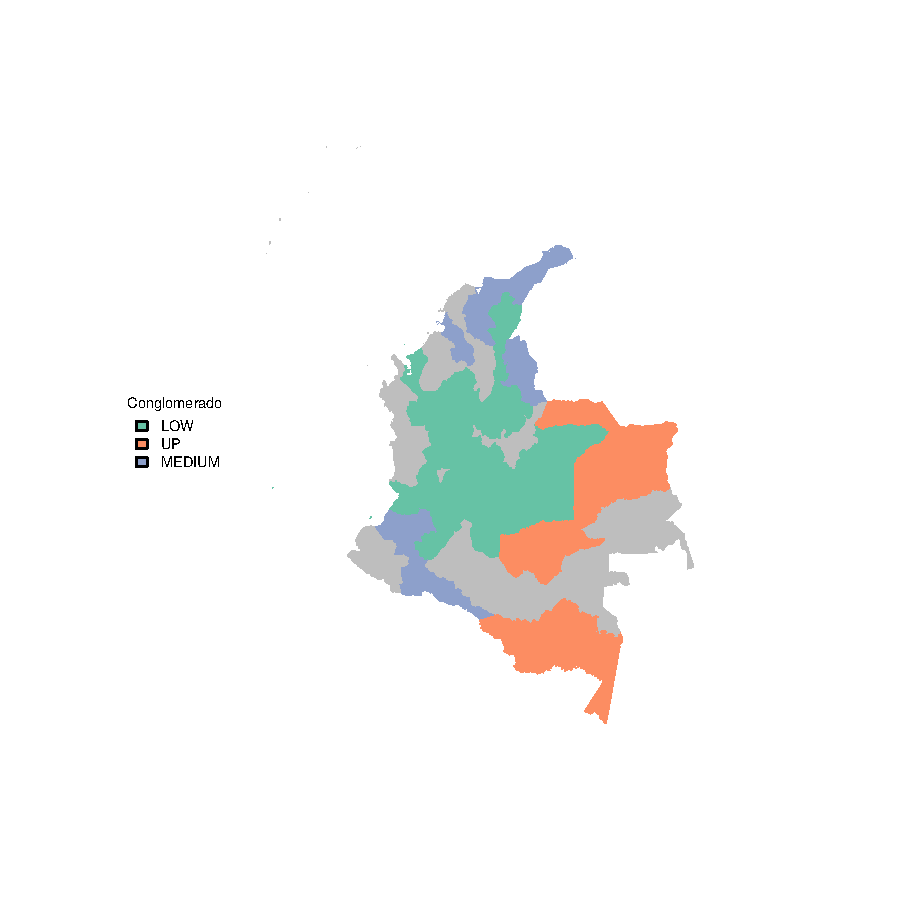
\includegraphics{ProyectoFinal-plotMapa}
\end{adjustbox}
\caption{Departamentos conglomerados según sus indicadores}\label{clustmap}
\end{figure}

\bibliographystyle{abbrv}
\renewcommand{\refname}{Bibliografia}
\bibliography{colombia}

\end{document}
